\documentclass{mcmthesis}
\mcmsetup{CTeX = true,   % 使用 CTeX 套装时,设置为 true
        tcn = 0000, problem = B,
        sheet = true, titleinsheet = true, keywordsinsheet = true,
        titlepage = false, abstract = true}
\usepackage{palatino}
\usepackage{lipsum}
\title{The \LaTeX{} Template for MCM Version \MCMversion}
\author{\small \href{http://www.latexstudio.net/}
  {
\includegraphics[width=7cm]{mcmthesis-logo}}}
\date{\today}
\begin{document}
\begin{abstract}
\lipsum[1]%写summary的地方
\begin{keywords}
keyword1; keyword2
\end{keywords}
\end{abstract}
\maketitle
\tableofcontents
\newpage

\section{Introduction}
\subsection{Background}

Lewis Mumford, a famous sociologist and literary critic,
once said in a metaphorical manner, ``Adding highway lanes
to deal with traffic congestion is like loosening your
belt to cure obesity.`` Fortunately, he did not experience
the worse congestion around today`s highway toll plaza.

Currently, with roaring number of vehicles, rising
construction costs and constrained available areas,
traffic jam becomes more and more serious but future
toll-plaza construction opportunities are limited to
improve this situation markedly. Figure 1 shows the
congestion in the toll plaza near Tappan Zee Bridge.

\begin{figure}[h]
\small
\centering
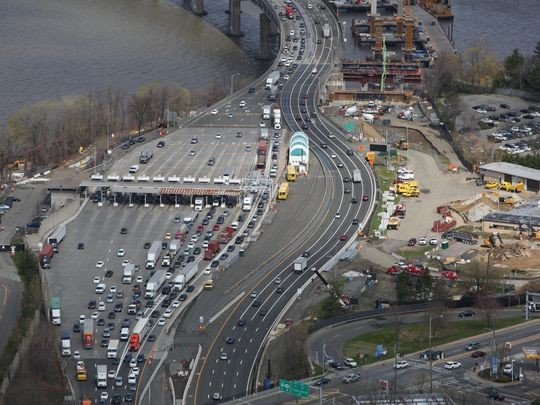
\includegraphics[width=10cm]{figure1}
\caption{Toll plaza congestion}\label{fig1}
\end{figure}

Subject to the constraints referred above, neither
increasing highway lanes nor building more tollbooths
seems practical enough to relieve traffic jam around a
toll plaza nowadays, particularly for some heavily-traveled
 roads such as the Garden State Parkway, New Jersey.
 Therefore, looking for some innovative design improvements
  on the geometric parameters of the extent toll plaza
  is an effective solution.


\subsection{Restatement of the Problem}
In this paper, we are required to explore if there is a
better-than-ever toll plaza model with specific shape,
size, and merging pattern. In this model, the prerequisite
is that vehicles fan in from B tollbooth egress lanes down
to L (B\textgreater L) lanes of traffic (i.e., the number of both
tollbooths and the lanes after merging are fixed). We aim
to construct a model that can optimize the arrangement
according to the following conditions.

\begin{itemize}
\item Enhance the capability of the accident prevention(A).
\item Maximize the throughput(T).
\item Minimize the cost of the land and road
construction(C).
\end{itemize}

Through our analysis, we determine if there are better
solutions than any toll plaza in common use. Afterwards,
the performance of our solution in light and heavy traffic
and other various situations along with corresponding
sensitivity analysis is discussed.

\subsection{Our Work}

\section{Assumptions}

\section{Notations}

\section{Model}
\subsection{Time Cost and Construction Cost}
\subsection{CA Model}

\section{Size}

\section{Shape}

\section{Merging Pattern}

\section{Conclusion}

\section{Sensitivity Analysis}
\subsection{The Performance of Our Solution in Light
and Heavy Traffic}
\subsection{Autonomous Vehicles}
\subsection{The Proportions of Different Tollbooths}

\section{Strengths and Weaknesses}
\subsection{Strengths}
\subsection{Weaknesses}

\begin{thebibliography}{99}
\bibitem{1} D. E. KNUTH   The \TeX{}book  the American
Mathematical Society and Addison-Wesley
Publishing Company , 1984-1986.
\bibitem{2}Lamport, Leslie,  \LaTeX{}: `` A Document Preparation System '',
Addison-Wesley Publishing Company, 1986.

\end{thebibliography}

\begin{appendices}

\section{First appendix}


Here are simulation programmes we used in our model as follow.\\

\textbf{\textcolor[rgb]{0.98,0.00,0.00}{Input matlab source:}}
\lstinputlisting[language=Matlab]{./code/mcmthesis-matlab1.m}

\section{Second appendix}

some more text \textcolor[rgb]{0.98,0.00,0.00}{\textbf{Input C++ source:}}
\lstinputlisting[language=C++]{./code/mcmthesis-sudoku.cpp}

\end{appendices}
\end{document}

%%
%% This work consists of these files mcmthesis.dtx,
%%                                   figures/ and
%%                                   code/,
%% and the derived files             mcmthesis.cls,
%%                                   mcmthesis-demo.tex,
%%                                   README,
%%                                   LICENSE,
%%                                   mcmthesis.pdf and
%%                                   mcmthesis-demo.pdf.
%%
%% End of file `mcmthesis-demo.tex'.
